% !Mode:: "TeX:UTF-8"
%%%%%%%%%%%%%%%%%%%%%%%%%%%%%%%%%%%%%%%%%%%%%%%%%%%%%%%%%%%%%%%%%%%%%%%%%%%%%%%%
%          ,
%      /\^/`\
%     | \/   |                CONGRATULATIONS!
%     | |    |             SPRING IS IN THE AIR!
%     \ \    /                                                _ _
%      '\\//'                                               _{ ' }_
%        ||                     hithesis v3                { `.!.` }
%        ||                                                ',_/Y\_,'
%        ||  ,                   dustincys                   {_,_}
%    |\  ||  |\          Email: yanshuoc@gmail.com             |
%    | | ||  | |            https://yanshuo.name             (\|  /)
%    | | || / /                                               \| //
%    \ \||/ /       https://github.com/dustincys/hithesis      |//
%      `\\//`   \\   \./    \\ /     //    \\./   \\   //   \\ |/ /
%     ^^^^^^^^^^^^^^^^^^^^^^^^^^^^^^^^^^^^^^^^^^^^^^^^^^^^^^^^^^^^^^
%%%%%%%%%%%%%%%%%%%%%%%%%%%%%%%%%%%%%%%%%%%%%%%%%%%%%%%%%%%%%%%%%%%%%%%%%%%%%%%%
\documentclass[type=bachelor]{hithesisbook}
% 此处选项中不要有空格
%%%%%%%%%%%%%%%%%%%%%%%%%%%%%%%%%%%%%%%%%%%%%%%%%%%%%%%%%%%%%%%%%%%%%%%%%%%%%%%%
% 必填选项
% type=doctor|master|bachelor|postdoc
%%%%%%%%%%%%%%%%%%%%%%%%%%%%%%%%%%%%%%%%%%%%%%%%%%%%%%%%%%%%%%%%%%%%%%%%%%%%%%%%
% 选填选项(选填选项的缺省值已经尽可能满足了大多数需求,除非明确知道自己有什么
% 需求)
% campus=shenzhen|weihai|harbin
%   含义:校区选项,默认harbin
% glue=true|false
%   含义:由于我工规范中要求字体行距在一个闭区间内,这个选项为true表示tex自
%   动选择,为false表示区间内一个最接近版心要求行数的要求的默认值,缺省值为
%   false。
% tocfour=true|false
%   含义:是否添加第四级目录,只对本科文科个别要求四级目录有效,缺省值为
%   false
% fontset=windows|mac|ubuntu|fandol|adobe
%   含义:设置字体,默认情况会自动识别系统,然后设置字体。后两个是开源字体,自行
%   下载安装后设置使用。windows是中易字库,窝工默认常用字体,绝对没毛病。mac和
%   ubuntu 默认分别是华文和思源字库,理论上用什么字库都行。后两种开源字库的安装
%   方法到谷歌上百度一下什么都有了。Linux非ubuntu发行版、非x86架构机器等如何运行
%   可到github issue上讨论。
% tocblank=true|false
%   含义:目录中第一章之前,是否加一行空白。缺省值为true。
% chapterhang=true|false
%   含义:目录的章标题是否悬挂居中,规范中要求章标题少于15字,所以这个选项
%   有无没什么用,除了特殊需求。缺省值为true。
% fulltime=true|false
%   含义:是否全日制,缺省值为true。非全日制如同等学力等,要在cover中设置类
%   型,封面中不同格式
% subtitle=true|false
%   含义:论文题目是否含有副标题,缺省值为false,如果有要在cover中设置副标
%   题内容,封面中显示。
% newgeometry=one|two
%   含义:规范中的自相矛盾之处,版芯是否包含页眉页脚,旧方法是按照包含页眉
%   页脚来设置。该选项是多选选项,如果没有这个选项,缺省值是旧模板的版芯设
%   置方法,如果设置该选项one或two,分别对应两种页眉页码对应版芯线的相对位
%   置。第一种是严格按照规范要求,难看。第二种微调了页眉页码位置,好一点。
% debug=true|false
%   含义:是否显示版芯框和行号,用来调试。默认否。
% openright=true|false
%   含义:博士论文是否要求章节首页必须在奇数页,此选项不在规范要求中,按个
%   人喜好自行决定。 默认否。注意,窝工的默认情况是打印版博士论文要求右翻页
%   ,电子版要求非右翻页且无空白页。如果想DIY(或身不由己DIY)在什么地方右
%   翻页,将这个选项设置为false,然后在目标位置添加`\cleardoublepage`命令即
%   可。
% library=true|false
%   含义:是否为提交到图书馆的电子版。默认否。注意:如果设置成true,那么
%   openright选项将被强制转换为false。
% capcenterlast=true|false
%   含义:图题、表题最后一行是否居中对齐(我工规范要求居中,但不要求居中对
%   齐),此选项不在规范要求中,按个人喜好自行决定。默认否。
% subcapcenterlast=true|false
%   含义:子图图题最后一行是否居中对齐(我工规范要求居中,但不要求居中对齐
%   ),此选项不在规范要求中,按个人喜好自行决定。默认否。
% absupper=true|false
%   含义:中文目录中的英文摘要在中文目录中的大小写样式歧义,在规范中要求首
%   字母大写,在work样例中是全大写。该选项控制是否全大写。默认否。
% bsmainpagenumberline=true|false
%   含义:由于本科生论文官方模板的页码和页眉格式混乱,提供这个选项自定义设
%   置是否在正文中显示页码横线,默认否。
% bsfrontpagenumberline=true|false
%   含义:由于本科生论文官方模板的页码和页眉格式混乱,提供这个选项自定义设
%   置是否在前文中显示页码横线,默认否。
% bsheadrule=true|false
%   含义:由于本科生论文官方模板的页码和页眉格式混乱,提供这个选项自定义设
%   置是否显示页眉横线,默认显示。
% splitbibitem=true|false
%   含义:参考文献每一个条目内能不能断页,应广大刀客要求添加。默认否。
% newtxmath=true|false
%   含义:数学字体是否使用新罗马。默认是。
% chapterbold=true|false
%   含义:本科生章标题在目录和正文中是否加粗
%%%%%%%%%%%%%%%%%%%%%%%%%%%%%%%%%%%%%%%%%%%%%%%%%%%%%%%%%%%%%%%%%%%%%%%%%%%%%%%%
\usepackage{hithesis}
\graphicspath{{figures/}}
\begin{document}
\frontmatter
% !Mode:: "TeX:UTF-8"

\hitsetup{
  %******************************
  % 注意:
  %   1. 配置里面不要出现空行
  %   2. 不需要的配置信息可以删除
  %******************************
  %
  %=====
  % 秘级
  %=====
  statesecrets={公开},
  natclassifiedindex={TM301.2},
  intclassifiedindex={62-5},
  %
  %=========
  % 中文信息
  %=========
  ctitleone={\large{基于C语言的RISC-V}},%本科生封面使用
  ctitletwo={\large{操作系统设计与实现}},%本科生封面使用
  ctitlecover={基于C语言的RISC-V操作系统设计与实现},%放在封面中使用,自由断行
  ctitle={基于C语言的RISC-V操作系统设计与实现},%放在原创性声明中使用
  % csubtitle={一条副标题}, %一般情况没有,可以注释掉
  cxueke={工学},
  csubject={计算机科学与技术},
  caffil={计算学部},
  cauthor={郭子阳},
  csupervisor={刘国军},
  % 日期自动使用当前时间,若需指定按如下方式修改:
  %cdate={2021年6月1日},
  cstudentid={1170300520},
  cnumber={no9527}, %编号
  %=========
  % 英文信息
  %=========
  etitle={Design and implementation of a C-based RISC-V operating system},
  % esubtitle={This is the sub title},
  exueke={Engineering},
  esubject={Computer Science and Technology},
  eaffil={\emultiline[t]{School of Computer Science \\ and Engineering}},
  eauthor={Guo Ziyang},
  esupervisor={Liu Guojun},
  % 日期自动生成,若需指定按如下方式修改:
  % edate={December, 2017},
  % estudenttype={Master of Art},
  %
  % 关键词用“英文逗号”分割
  ckeywords={RISC-V, 操作系统, 内存管理,ELF文件, 文件系统, 壳(shell)},
  ekeywords={RISC-V, operating system, memory management, ELF file, file system, shell},
}

\begin{cabstract}

指令集架构(ISA)是计算机的一种抽象模型,是计算机体系结构模型中与程序设计相关的部分,也是处理器的灵魂。现阶段市场上常见的ISA,如x86和ARM,都是商业闭源的,不利于二次开发。于是RISC-V一出现,就受到了各大研究机构和高校的青睐。同样,这款完全开源的指令集架构,也有助于解决我国当前面临的芯片困境,进一步反哺国内生态,尤其是操作系统方面,以保障我国在核心产业的自主可控。

尽管RISC-V已经出现多年,国内对它的研究却一直局限于嵌入式和移动设备领域,同时,对于RISC-V指令集架构的通用操作系统的研究,相关资料较少且专业性过强,成为阻碍其进入高校研究和课堂教学的重要因素。

为了解决上述问题,进一步推动RISC-V在高校教学中的沉淀,促进RISC-V的传播,本论文讨论了一种基于C语言的RISC-V操作系统的设计,基于模块对整个工程进行划分,随后进一步细化了各个模块的具体设计,譬如中断的模式、线程调度算法等,并主要给出各个模块的实现细节,最后针对此操作系统,给出了一份比较详细的实现文档。本文实现的操作系统主要分为四个模块:中断管理、内存管理、线程调度和文件系统。中断模块主要用于处理环境调用,同时处理定时器中断来辅助线程调度;内存管理模块对操作系统的可用物理内存进行管理分配,内存管理以两个粒度进行:动态内存分配和按页分配,并实现虚拟内存以进行进程间的代码数据隔离;线程调度保证了所有正在运行的线程都有平等使用CPU的机会,并根据需要动态挂起和唤醒线程;文件系统对操作系统开放了一个统一的文件读写接口,使得不同类型的文件实现细节对操作系统来说是透明的。

本文设计实现的基于C语言的RISC-V操作系统,结构清晰,方便横向扩展。同时代码规范,注释和文档完整详细,可用于教学用途,并可以在客观上推动RISC-V开源社区的发展。

\end{cabstract}

\begin{eabstract}

Instruction Set Architecture (ISA) is an abstract model of computer, a part of computer architecture model related to programming, and also the soul of the processor. Currently, common ISA such as x86 and ARM, are commercial closed source, which is not conducive to secondary development. As soon as RISC-V appeared, it was favored by various research institutions and universities. In the same way, this completely open source instruction set architecture will also help solve China's current chip dilemma and further feed the domestic ecology, especially in the aspect of operating system, so as to guarantee China's autonomy and control in the core industry.

Although RISC-V has been brought up for many years, domestic research on RISC-V has been limited to the field of embedded and mobile devices. At the same time, for the research on RISC-V general operating system, there are few relevant materials and it is too specialized, which has become an important factor hindering its entry into university research and classroom teaching.

In order to solve the above problems, further promote the participation of RISC-V in college teaching and promote the spread of RISC-V, this paper discusses a RISC-V operating system based on C language design. This paper first divides the whole project based on modules, then further discusses the specific design of each module, such as interrupt mode, thread scheduling, etc., and gives the implementation details of each module. Finally, a detailed implementation document is given for this operating system. The operating system realized in this paper is mainly divided into four modules: interrupt management, memory management, thread scheduling and file system. The interrupt management module is mainly used to handle the environment call and timer interrupt to assist thread scheduling. The memory management module manages and allocates the physical memory the system can use. The memory management is carried out in two granularity: dynamic memory allocation and page-based allocation, and the virtual memory is realized to isolate the code and data between processes. Thread scheduling ensures that all running threads have equal access to CPU, and dynamically suspends and awakens threads as needed. The file system provides a unified file reading and writing interface to the operating system, making the implementation details of different types of files transparent to the operating system.

The RISC-V operating system based on C language designed and implemented in this paper has a clear structure and is convenient for horizontal expansion. At the same time, the code conforms to the specification, the comments and documentation are comprehensive and detailed, so as to be used for educational purposes. And it can objectively promote the development of RISC-V open source community.

\end{eabstract}
 % 封面
\makecover
%\begin{denotation}
\begin{table}[h]%此处最好是h
\caption{国际单位制中具有专门名称的导出单位}
\vspace{0.5em}\centering\wuhao
\begin{tabular}{ccccc}
\toprule[1.5pt]
量的名称&单位名称&单位符号&其它表示实例\\
\midrule[1pt]
频率&赫[兹]&Hz&s-1\\
\bottomrule[1.5pt]
\end{tabular}
\end{table}
\end{denotation}
%物理量名称表,符合规范为主,有要求添加
\tableofcontents %目录
\mainmatter
% !Mode:: "TeX:UTF-8"

\chapter[哈尔滨工业大学研究生学位论文撰写规范]{哈尔滨工业大学研究生学
  位论文\protect\\撰写规范}[Harbin Institute of Technology Postgraduate Dissertation Writing Specifications]

研究生学位论文是研究生科学研究工作的全面总结,是描述其研究成果、代表其研究水平的
重要学术文献资料,是申请和授予相应学位的基本依据。学位论文撰写是研究生培养过程的
基本训练之一,必须按照确定的规范认真执行。研究生应严肃认真地撰写学位论文,指导教
师应加强指导,严格把关。

学位论文撰写应实事求是,杜绝造假和抄袭等行为;应符合国家及各专业部门制定的有关标
准,符合汉语语法规范。硕士和博士学位论文,除在字数、理论研究的深度及创造性成果等
方面的要求不同外,撰写规范要求基本一致。人文与社会科学、管理学科可在本撰写规范的
基础上补充制定专业的学术规范。

\section{内容要求}[Content specification]
\subsection{题目}[Title]

题目应以简明的词语,恰当、准确、科学地反映论文最重要的特定内容(一般不超过25字),
应中英文对照。题目通常由名词性短语构成,不能含有标点符号;应尽量避免使用不常用的
缩略词、首字母缩写字、字符、代号和公式等。

如题目内容层次很多,难以简化时,可采用题目和副题目相结合的方法。题目与副题目字数
之和不应超过35字,中文的题目与副题目之间用破折号相连,英文则用冒号相连。副题目起
补充、阐明题目的作用。题目和副题目在整篇学位论文中的不同地方出现时,应保持一致。

\subsection{摘要与关键词}[Abstraction and key words]
\subsubsection{摘要}[Abstraction]

摘要是论文内容的高度概括,应具有独立性和自含性,即不阅读论文的全文,就能通过摘要
了解整个论文的必要信息。摘要应包括本论文研究的目的、理论与实际意义、主要研究内容、
研究方法等,重点突出研究成果和结论。

摘要的内容要完整、客观、准确,应做到不遗漏、不拔高、不添加。摘要应按层次逐段简要
写出,避免将摘要写成目录式的内容介绍。摘要在叙述研究内容、研究方法和主要结论时,
除作者的价值和经验判断可以使用第一人称外,一般使用第三人称,采用“分析了……原因”、
“认为……”、“对……进行了探讨”等记述方法进行描述。避免主观性的评价意见,避免
对背景、目的、意义、概念和一般性(常识性)理论叙述过多。

摘要需采用规范的名词术语(包括地名、机构名和人名)。对个别新术语或无中文译文的术
语,可用外文或在中文译文后加括号注明外文。摘要中不宜使用公式、化学结构式、图表、
非常用的缩写词和非公知公用的符号与术语,不标注引用文献编号。

博士学位论文摘要应包括以下几个方面的内容:

(1)论文的研究背景及目的。简洁准确地交代论文的研究背景与意义、相关领域的研究现
状、论文所针对的关键科学问题,使读者把握论文选题的必要性和重要性。此部分介绍不宜
写得过多,一般不多于400字。

(2)论文的主要研究内容。介绍论文所要解决核心问题开展的主要研究工作以及研究方法
或研究手段,使读者可以了解论文的研究思路、研究方案、研究方法或手段的合理性与先进
性。

(3)论文的主要创新成果。简要阐述论文的新思想、新观点、新技术、新方法、新结论等
主要信息,使读者可以了解论文的创新性。

(4)论文成果的理论和实际意义。客观、简要地介绍论文成果的理论和实际意义,使读者
可以快速获得论文的学术价值。

\subsubsection{关键词}[Keywords]
关键词是供检索用的主题词条。关键词应集中体现论文特色,反映研究成果的内涵,具有语
义性,在论文中有明确的出处,并应尽量采用《汉语主题词表》或各专业主题词表提供的规
范词,应列取3$\sim$6个关键词,按词条的外延层次从大到小排列。

\subsection{目录}[Content]

论文中各章节的顺序排列表,包括论文中全部章、节、条三级标题及其页码。

\subsection{论文正文}[Main body]

论文正文包括绪论、论文主体及结论等部分。

\subsubsection{绪论}
绪论一般作为第1章。绪论应包括:本研究课题的来源、背景及其理论意义与实际意义;国
内外与课题相关研究领域的研究进展及成果、存在的不足或有待深入研究的问题,归纳出将
要开展研究的理论分析框架、研究内容、研究程序和方法。

绪论部分要注意对论文所引用国内外文献的准确标注。绪论的主要研究内容的撰写宜使用将
来时态,切忌将论文目录直接作为研究内容。

\subsubsection{论文主体}
论文主体是学位论文的主要部分,应该结构严谨,层次清晰,重点突出,文字简练、通顺。
论文各章之间应该前后关联,构成一个有机的整体。论文给出的数据必须真实可靠,推理正
确,结论明确,无概念性和科学性错误。对于科学实验、计算机仿真的条件、实验过程、仿
真过程等需加以叙述,避免直接给出结果、曲线和结论。引用他人研究成果或采用他人成说
时,应注明出处,不得将其与本人提出的理论分析混淆在一起。

论文主体各章后应有一节“本章小结”,实验方法或材料等章节可不写“本章小结”。各章
小结是对各章研究内容、方法与成果的简洁准确的总结与概括,也是论文最后结论的依据。

\subsubsection{结论}
结论作为学位论文正文的组成部分,单独排写,不加章标题序号,不标注




% Local Variables:
% TeX-master: "../main"
% TeX-engine: xetex
% End:
% !Mode:: "TeX:UTF-8"

\chapter{绪论}[Introduction]

\section{课题来源及研究的目的和意义}

指令集架构(ISA),是计算机的一种抽象模型,是计算机体系结构模型中与程序设计相关的部分。通常,指令集架构定义了一系列支持的数据类型、寄存器、内存管理、基本特性与IO模型。计算机处理器的指令集架构有以下常见的两种:复杂指令集架构(CISC)、精简指令集架构(RISC),前者的代表就是x86架构,而后者的代表就是ARM架构。无论如何划分,不可否认的是,当今最流行的几个指令集架构,如x86和ARM,都是商业闭源的,在使用这些指令集架构时,需要向Intel或ARM控股缴纳高额的许可费。但是,Krste Asanović等人提出了这样一个观点:指令集架构应当是开放的,并以RISC-V作为开源指令集架构的典型进行论述。

RISC-V是一个基于精简指令集原则的开源指令集架构,该项目2010年始于加州大学伯克利分校,但是该项目的贡献者更多的是校外的志愿者和行业工作者。尽管不是第一个开源指令集,但是由于RISC-V适用于各种设备,譬如云计算机、PC机、移动设备和嵌入式系统,且其开源免费的特性使得它的社区十分活跃。于是RISC-V架构一经出现,就有许多芯片设计者以此为架构设计SoC。

相较于以功耗低著称的ARM架构处理器,RISC-V性能更强、面积更小、功耗更低,且相对于ARM,指令更加丰富,可扩展性更强,并且开源免费。或许是感受到了来自RISC-V的巨大压力,ARM控股甚至上线了一个网站来专门质疑RISC-V指令集。而相对于Intel的x86指令集架构,RISC-V没有那么多的历史包袱,不需要考虑向后兼容问题,可以说是“轻装上阵”,在设计操作系统时就无须考虑类似“A20地址线”的问题。而在关键技术被其他国家卡脖子的当今中国,开源免费的RISC-V可能有助于我国打破芯片壁垒。

同时,随着我国逐渐重视核心技术国有化,保障我国核心产业自主可控,我国开始大力发展自研芯片和自研操作系统。然而,相关工作大都是在企业和研究院层面展开,并没有下沉到高校层面的,形成了产学断层。这使得对于RISC-V相关技术的研究和教学,如RISC-V架构的芯片和支持RISC-V的操作系统的相关方向,成为国内高校研学的一片空白地带。

目前,大部分高校的操作系统的课程,都是基于x86架构设计的。然而,x86架构向后兼容的特性,使得即使是较新的x86操作系统,也不得不兼容一些过时的、已经被废弃不用的特性,例如上文提到的A20地址线。这使得学生对于操作系统本身的概念,会和x86一些特性混淆。令学生可能会更专注于繁琐而多余的x86特性,而不是聚焦于操作系统领域的通用概念。而RISC-V架构的操作系统,由于架构本身的精巧轻盈,更能让学生着眼于系统自身的设计。

基于以上原因,本文讨论了一种基于C语言和RISC-V架构的操作系统的设计方案,并给出其实现代码,旨在推动RISC-V向高校课程和实验室的下沉,以期能够反哺开源社区,最终客观上促进社区发展和RISC-V在国内的传播。

\section{国内外研究现状及分析}

\section{研究内容与方案}
\backmatter
% !Mode:: "TeX:UTF-8" 
\begin{conclusions}

学位论文的结论作为论文正文的最后一章单独排写,但不加章标题序号。

结论应是作者在学位论文研究过程中所取得的创新性成果的概要总结,不能与摘要混为一谈。博士学位论文结论应包括论文的主要结果、创新点、展望三部分,在结论中应概括论文的核心观点,明确、客观地指出本研究内容的创新性成果(含新见解、新观点、方法创新、技术创新、理论创新),并指出今后进一步在本研究方向进行研究工作的展望与设想。对所取得的创新性成果应注意从定性和定量两方面给出科学、准确的评价,分(1)、(2)、(3)…条列出,宜用“提出了”、“建立了”等词叙述。

\end{conclusions}
   % 结论
\bibliographystyle{hithesis} %如果没有参考文献时候
\bibliography{reference}
%%%%%%%%%%%%%%%%%%%%%%%%%%%%%%%%%%%%%%%%%%%%%%%%%%%%%%%%%%%%%%%%%%%%%%%%%%%%%%%% 
%-- 注意:以下本硕博、博后书序不一致 --%
%%%%%%%%%%%%%%%%%%%%%%%%%%%%%%%%%%%%%%%%%%%%%%%%%%%%%%%%%%%%%%%%%%%%%%%%%%%%%%%% 
% 硕博书序
%%%%%%%%%%%%%%%%%%%%%%%%%%%%%%%%%%%%%%%%%%%%%%%%%%%%%%%%%%%%%%%%%%%%%%%%%%%%%%%% 
\begin{appendix}%附录
% -*-coding: utf-8 -*-
%%%%%%%%%%%%%%%%%%%%%%%%%%%%%%%%%%%%%%%%%%%%%%%%%%%%%%%%%
\chapter{带章节的附录}[Full Appendix]%
完整的附录内容,包含章节,公式,图表等

%%%%%%%%%%%%%%%%%%%%%%%%%%%%%%%%%%%%%%%%%%%%%%%%%%%%%%%%%
\section{附录节的内容}[Section in Appendix]
这是附录的节的内容

附录中图的示例:
\begin{figure}[htbp]
\centering
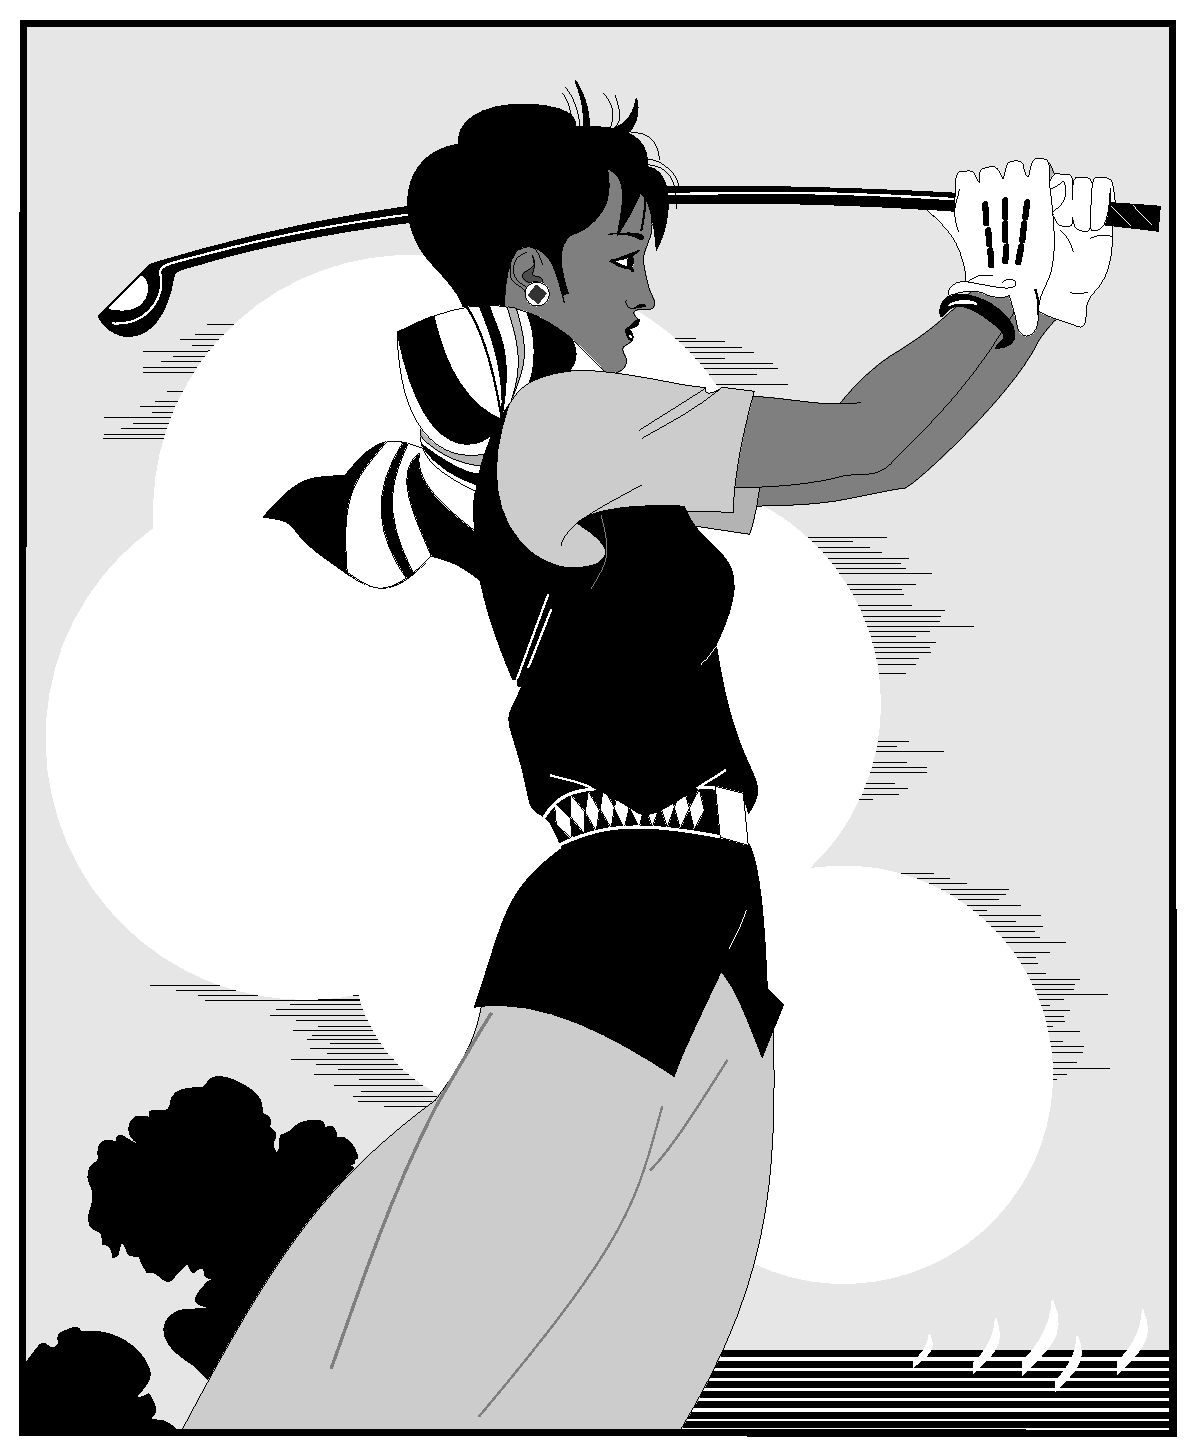
\includegraphics[width = 0.4\textwidth]{golfer}
%\bicaption[golfer5]{}{\xiaosi[0]打高尔夫球的人}{Fig.$\!$}{The person playing golf}\vspace{-1em}
\caption{\xiaosi[0]打高尔夫球的人}
\end{figure}

附录中公式的示例:
\begin{align}
a & = b \times c \\
E & = m c^2
\label{eq}
\end{align}

\chapter{这个星球上最好的免费Linux软件列表}[List of the Best Linux Software in our Planet]
\section{系统}

\href{http://fvwm.org/}{FVWM 自从上世纪诞生以来,此星球最强大的窗口管理器。}
推荐基于FVWM的桌面设计hifvwm:\href{https://github.com/dustincys/hifvwm}{https://github.com/dustincys/hifvwm}。

\subsection{hifvwm的优点}

\begin{enumerate}
	\item 即使打开上百个窗口也不会“蒙圈”。计算机性能越来越强大,窗口任务的管理必须要升级到打怪兽级别。
	\item 自动同步Bing搜索主页的壁纸。每次电脑开机,午夜零点自动更新,用户
		也可以手动更新,从此审美再也不疲劳。
	\item 切换窗口自动聚焦到最上面的窗口。使用键盘快捷键切换窗口时候,减少
		操作过程,自动聚焦到目标窗口。这一特性是虚拟窗口必须的人性化设
		计。
	\item 类似window右下角的功能的最小化窗口来显示桌面的功能此处类似
		win7/win10,实现在一个桌面之内操作多个任务。
	\item 任务栏结合标题栏。采用任务栏和标题栏结合,节省空间。
	\item 同类窗口切换。可以在同类窗口之内类似alt-tab的方式切换。
	\item ……
\end{enumerate}

\section{其他}

\href{https://github.com/goldendict/goldendict}{goldendict 星球最强大的桌面字典。}

\href{https://github.com/yarrick/iodine}{iodine,“HIT-WLAN + 锐捷”时代的福音。}

\href{http://www.aircrack-ng.org/}{aircrack,Wifi“安全性评估”工具。}

\href{https://www.ledger-cli.org/}{ledger,前“金融区块链”时代最好的复式记账系统。}

\href{https://orgmode.org/}{orgmode,最强大的笔记系统,从来没有之一。}

\href{https://www.jianguoyun.com/}{坚果云,国内一款支持WebDav的云盘系统,国内真正的云盘没有之一。}

\href{http://www.mutt.org/}{mutt, ``All mail clients suck. This one just sucks less.''}

\section{vim}
实现中英文每一句一行,以及实现每一句折叠断行的简单正则式,tex源码更加乖乖。
\begin{lstlisting}
vnoremap <leader>fae J:s/[.!?]\zs\s\+/\="\r".matchstr(getline('.'), '^\s*')/g<CR>
vnoremap <leader>fac J:s/[。!?]/\=submatch(0)."\n".matchstr(getline('.'), '^\s*')/g<CR>
vnoremap <leader>fle :!fmt -80 -s<CR>
\end{lstlisting}

\end{appendix}
% !Mode:: "TeX:UTF-8" 
\begin{publication}
\noindent\textbf{发表的相关论文}
\begin{publist}
\item	XXX,XXX. Static Oxidation Model of Al-Mg/C Dissipation Thermal Protection Materials[J]. Rare Metal Materials and Engineering, 2010, 39(Suppl. 1): 520-524.(SCI~收录,IDS号为~669JS,IF=0.16)
\item XXX,XXX. 精密超声振动切削单晶铜的计算机仿真研究[J]. 系统仿真学报,2007,19(4):738-741,753.(EI~收录号:20071310514841)
\item XXX,XXX. 局部多孔质气体静压轴向轴承静态特性的数值求解[J]. 摩擦学学报,2007(1):68-72.(EI~收录号:20071510544816)
\item XXX,XXX. 硬脆光学晶体材料超精密切削理论研究综述[J]. 机械工程学报,2003,39(8):15-22.(EI~收录号:2004088028875)
\item XXX,XXX. 基于遗传算法的超精密切削加工表面粗糙度预测模型的参数辨识以及切削参数优化[J]. 机械工程学报,2005,41(11):158-162.(EI~收录号:2006039650087)
\item XXX,XXX. Discrete Sliding Mode Cintrok with Fuzzy Adaptive Reaching Law on 6-PEES Parallel Robot[C]. Intelligent System Design and Applications, Jinan, 2006: 649-652.(EI~收录号:20073210746529)
\end{publist}

\noindent\textbf{(二)申请及已获得的专利(无专利时此项不必列出)}
\begin{publist}
\item XXX,XXX. 一种温热外敷药制备方案:中国,88105607.3[P]. 1989-07-26.
\end{publist}

\noindent\textbf{(三)参与的科研项目及获奖情况}
\begin{publist}
\item	XXX,XXX. XX~气体静压轴承技术研究, XX~省自然科学基金项目.课题编号:XXXX.
\item XXX,XXX. XX~静载下预应力混凝土房屋结构设计统一理论. 黑江省科学技术二等奖, 2007.
\end{publist}
%\vfill
%\hangafter=1\hangindent=2em\noindent
%\setlength{\parindent}{2em}
\end{publication}
    % 所发文章
\begin{ceindex}
  %如果想要手动加索引,注释掉以下这一样,用wordlist环境
\printsubindex*
\end{ceindex}
    % 索引, 根据自己的情况添加或者不添加,选择自动添加或者手工添加。
\authorization %授权
%\authorization[saomiao.pdf] %添加扫描页的命令,与上互斥
% !Mode:: "TeX:UTF-8"
\begin{acknowledgements}

Moonix操作系统和本论文是在刘国军老师的指导下完成的。刘国军老师教授的操作系统课程,使我对操作系统的设计与实现产生了浓厚的兴趣,并最终促成的我的选题。在项目进行过程中,刘国军老师渊博的专业知识和悉心的指导,使得我能够最终完成这个项目。在此,谨向刘国军老师致以最诚挚的谢意。

感谢大学期间所有教过我的老师们,你们严谨的治学精神、渊博的专业知识,培养了我对计算机科学浓厚的兴趣,非常感谢。

感谢我的女朋友。很多时候,我都疲于学业和工作,没法常伴她左右,她也不曾有一丝怨言。Moonix操作系统就是以她的名字命名的,以表达我对她的谢意。这一点我一直没好意思告诉刘国军老师。

感谢我的父母给予我无私的关心和照顾,没有你们的照顾和支持,就不会有我的今天,我永远无法回报你们对我的爱,所以我希望能顺利完成学业,给你们一点欣慰。

感谢所有帮助过我的老师、同学和朋友,没有你们的帮助,就没有我今天的成绩。

感谢字节跳动的同事们,本论文是在字节跳动实习期间完成的,感谢他们对于我摸鱼写论文和频繁请假的包容。你们开放谦逊、坦诚清晰的字节范儿,使得我对未来的工作充满的期待,很荣幸能和你们成为同事。

最后再次感谢所有帮助过我的老师、家人、同学和朋友们!

\end{acknowledgements}
 %致谢
% !Mode:: "TeX:UTF-8" 

\begin{resume}
XXXX~年~XX~月~XX~日出生于~XXXX。

XXXX~年~XX~月考入~XX~大学~XX~院(系)XX~专业,XXXX~年~XX~月本科毕业并获得~XX~学学士学位。

XXXX~年~XX~月------XXXX~年~XX~月在~XX~大学~XX~院(系)XX~学科学习并获得~XX~学硕士学位。

XXXX~年~XX~月------XXXX~年~XX~月在~XX~大学~XX~院(系)XX~学科学习并获得~XX~学博士学位。

获奖情况:如获三好学生、优秀团干部、X~奖学金等(不含科研学术获奖)。

工作经历:

\textbf{( 除全日制硕士生以外,其余学生均应增列此项。个人简历一般应包含教育经历和工作经历。)}
\end{resume}
          % 博士学位论文有个人简介
%%%%%%%%%%%%%%%%%%%%%%%%%%%%%%%%%%%%%%%%%%%%%%%%%%%%%%%%%%%%%%%%%%%%%%%%%%%%%%%% 
% 本科书序为:
%%%%%%%%%%%%%%%%%%%%%%%%%%%%%%%%%%%%%%%%%%%%%%%%%%%%%%%%%%%%%%%%%%%%%%%%%%%%%%%% 
% \authorization %授权
% % \authorization[saomiao.pdf] %添加扫描页的命令,与上互斥
% % !Mode:: "TeX:UTF-8"
\begin{acknowledgements}

Moonix操作系统和本论文是在刘国军老师的指导下完成的。刘国军老师教授的操作系统课程,使我对操作系统的设计与实现产生了浓厚的兴趣,并最终促成的我的选题。在项目进行过程中,刘国军老师渊博的专业知识和悉心的指导,使得我能够最终完成这个项目。在此,谨向刘国军老师致以最诚挚的谢意。

感谢大学期间所有教过我的老师们,你们严谨的治学精神、渊博的专业知识,培养了我对计算机科学浓厚的兴趣,非常感谢。

感谢我的女朋友。很多时候,我都疲于学业和工作,没法常伴她左右,她也不曾有一丝怨言。Moonix操作系统就是以她的名字命名的,以表达我对她的谢意。这一点我一直没好意思告诉刘国军老师。

感谢我的父母给予我无私的关心和照顾,没有你们的照顾和支持,就不会有我的今天,我永远无法回报你们对我的爱,所以我希望能顺利完成学业,给你们一点欣慰。

感谢所有帮助过我的老师、同学和朋友,没有你们的帮助,就没有我今天的成绩。

感谢字节跳动的同事们,本论文是在字节跳动实习期间完成的,感谢他们对于我摸鱼写论文和频繁请假的包容。你们开放谦逊、坦诚清晰的字节范儿,使得我对未来的工作充满的期待,很荣幸能和你们成为同事。

最后再次感谢所有帮助过我的老师、家人、同学和朋友们!

\end{acknowledgements}
 %致谢
% \begin{appendix}%附录
% \chapter{外文资料原文}
\label{cha:engorg}

\title{The title of the English paper}

\textbf{Abstract:} As one of the most widely used techniques in operations
research, \emph{ mathematical programming} is defined as a means of maximizing a
quantity known as \emph{bjective function}, subject to a set of constraints
represented by equations and inequalities. Some known subtopics of mathematical
programming are linear programming, nonlinear programming, multiobjective
programming, goal programming, dynamic programming, and multilevel
programming$^{[1]}$.

It is impossible to cover in a single chapter every concept of mathematical
programming. This chapter introduces only the basic concepts and techniques of
mathematical programming such that readers gain an understanding of them
throughout the book$^{[2,3]}$.


\section{Single-Objective Programming}
The general form of single-objective programming (SOP) is written
as follows,
\begin{equation}\tag*{(123)} % 如果附录中的公式不想让它出现在公式索引中,那就请
                             % 用 \tag*{xxxx}
\left\{\begin{array}{l}
\max \,\,f(x)\\[0.1 cm]
\mbox{subject to:} \\ [0.1 cm]
\qquad g_j(x)\le 0,\quad j=1,2,\cdots,p
\end{array}\right.
\end{equation}
which maximizes a real-valued function $f$ of
$x=(x_1,x_2,\cdots,x_n)$ subject to a set of constraints.

\newtheorem{mpdef}{Definition}[chapter]
\begin{mpdef}
In SOP, we call $x$ a decision vector, and
$x_1,x_2,\cdots,x_n$ decision variables. The function
$f$ is called the objective function. The set
\begin{equation}\tag*{(456)} % 这里同理,其它不再一一指定。
S=\left\{x\in\Re^n\bigm|g_j(x)\le 0,\,j=1,2,\cdots,p\right\}
\end{equation}
is called the feasible set. An element $x$ in $S$ is called a
feasible solution.
\end{mpdef}

\newtheorem{mpdefop}[mpdef]{Definition}
\begin{mpdefop}
A feasible solution $x^*$ is called the optimal
solution of SOP if and only if
\begin{equation}
f(x^*)\ge f(x)
\end{equation}
for any feasible solution $x$.
\end{mpdefop}

One of the outstanding contributions to mathematical programming was known as
the Kuhn-Tucker conditions\ref{eq:ktc}. In order to introduce them, let us give
some definitions. An inequality constraint $g_j(x)\le 0$ is said to be active at
a point $x^*$ if $g_j(x^*)=0$. A point $x^*$ satisfying $g_j(x^*)\le 0$ is said
to be regular if the gradient vectors $\nabla g_j(x)$ of all active constraints
are linearly independent.

Let $x^*$ be a regular point of the constraints of SOP and assume that all the
functions $f(x)$ and $g_j(x),j=1,2,\cdots,p$ are differentiable. If $x^*$ is a
local optimal solution, then there exist Lagrange multipliers
$\lambda_j,j=1,2,\cdots,p$ such that the following Kuhn-Tucker conditions hold,
\begin{equation}
\label{eq:ktc}
\left\{\begin{array}{l}
    \nabla f(x^*)-\sum\limits_{j=1}^p\lambda_j\nabla g_j(x^*)=0\\[0.3cm]
    \lambda_jg_j(x^*)=0,\quad j=1,2,\cdots,p\\[0.2cm]
    \lambda_j\ge 0,\quad j=1,2,\cdots,p.
\end{array}\right.
\end{equation}
If all the functions $f(x)$ and $g_j(x),j=1,2,\cdots,p$ are convex and
differentiable, and the point $x^*$ satisfies the Kuhn-Tucker conditions
(\ref{eq:ktc}), then it has been proved that the point $x^*$ is a global optimal
solution of SOP.

\subsection{Linear Programming}
\label{sec:lp}

If the functions $f(x),g_j(x),j=1,2,\cdots,p$ are all linear, then SOP is called
a {\em linear programming}.

The feasible set of linear is always convex. A point $x$ is called an extreme
point of convex set $S$ if $x\in S$ and $x$ cannot be expressed as a convex
combination of two points in $S$. It has been shown that the optimal solution to
linear programming corresponds to an extreme point of its feasible set provided
that the feasible set $S$ is bounded. This fact is the basis of the {\em simplex
  algorithm} which was developed by Dantzig as a very efficient method for
solving linear programming.
\begin{table}[ht]
\centering
  \centering
  \caption*{Table~1\hskip1em This is an example for manually numbered table, which
    would not appear in the list of tables}
  \label{tab:badtabular2}
  \begin{tabular}[c]{|m{1.5cm}|c|c|c|c|c|c|}\hline
    \multicolumn{2}{|c|}{Network Topology} & \# of nodes &
    \multicolumn{3}{c|}{\# of clients} & Server \\\hline
    GT-ITM & Waxman Transit-Stub & 600 &
    \multirow{2}{2em}{2\%}&
    \multirow{2}{2em}{10\%}&
    \multirow{2}{2em}{50\%}&
    \multirow{2}{1.2in}{Max. Connectivity}\\\cline{1-3}
    \multicolumn{2}{|c|}{Inet-2.1} & 6000 & & & &\\\hline
    & \multicolumn{2}{c|}{ABCDEF} &\multicolumn{4}{c|}{} \\\hline
\end{tabular}
\end{table}

Roughly speaking, the simplex algorithm examines only the extreme points of the
feasible set, rather than all feasible points. At first, the simplex algorithm
selects an extreme point as the initial point. The successive extreme point is
selected so as to improve the objective function value. The procedure is
repeated until no improvement in objective function value can be made. The last
extreme point is the optimal solution.

\subsection{Nonlinear Programming}

If at least one of the functions $f(x),g_j(x),j=1,2,\cdots,p$ is nonlinear, then
SOP is called a {\em nonlinear programming}.

A large number of classical optimization methods have been developed to treat
special-structural nonlinear programming based on the mathematical theory
concerned with analyzing the structure of problems.

Now we consider a nonlinear programming which is confronted solely with
maximizing a real-valued function with domain $\Re^n$.  Whether derivatives are
available or not, the usual strategy is first to select a point in $\Re^n$ which
is thought to be the most likely place where the maximum exists. If there is no
information available on which to base such a selection, a point is chosen at
random. From this first point an attempt is made to construct a sequence of
points, each of which yields an improved objective function value over its
predecessor. The next point to be added to the sequence is chosen by analyzing
the behavior of the function at the previous points. This construction continues
until some termination criterion is met. Methods based upon this strategy are
called {\em ascent methods}, which can be classified as {\em direct methods},
{\em gradient methods}, and {\em Hessian methods} according to the information
about the behavior of objective function $f$. Direct methods require only that
the function can be evaluated at each point. Gradient methods require the
evaluation of first derivatives of $f$. Hessian methods require the evaluation
of second derivatives. In fact, there is no superior method for all
problems. The efficiency of a method is very much dependent upon the objective
function.

\subsection{Integer Programming}

{\em Integer programming} is a special mathematical programming in which all of
the variables are assumed to be only integer values. When there are not only
integer variables but also conventional continuous variables, we call it {\em
  mixed integer programming}. If all the variables are assumed either 0 or 1,
then the problem is termed a {\em zero-one programming}. Although integer
programming can be solved by an {\em exhaustive enumeration} theoretically, it
is impractical to solve realistically sized integer programming problems. The
most successful algorithm so far found to solve integer programming is called
the {\em branch-and-bound enumeration} developed by Balas (1965) and Dakin
(1965). The other technique to integer programming is the {\em cutting plane
  method} developed by Gomory (1959).

\hfill\textit{Uncertain Programming\/}\quad(\textsl{BaoDing Liu, 2006.2})

\section*{References}
\noindent{\itshape NOTE: These references are only for demonstration. They are
  not real citations in the original text.}

\begin{translationbib}
\item Donald E. Knuth. The \TeX book. Addison-Wesley, 1984. ISBN: 0-201-13448-9
\item Paul W. Abrahams, Karl Berry and Kathryn A. Hargreaves. \TeX\ for the
  Impatient. Addison-Wesley, 1990. ISBN: 0-201-51375-7
\item David Salomon. The advanced \TeX book.  New York : Springer, 1995. ISBN:0-387-94556-3
\end{translationbib}

\chapter{外文资料的调研阅读报告或书面翻译}

\title{英文资料的中文标题}

{\heiti 摘要:} 本章为外文资料翻译内容。如果有摘要可以直接写上来,这部分好像没有
明确的规定。

\section{单目标规划}
北冥有鱼,其名为鲲。鲲之大,不知其几千里也。化而为鸟,其名为鹏。鹏之背,不知其几
千里也。怒而飞,其翼若垂天之云。是鸟也,海运则将徙于南冥。南冥者,天池也。
\begin{equation}\tag*{(123)}
 p(y|\mathbf{x}) = \frac{p(\mathbf{x},y)}{p(\mathbf{x})}=
\frac{p(\mathbf{x}|y)p(y)}{p(\mathbf{x})}
\end{equation}

吾生也有涯,而知也无涯。以有涯随无涯,殆已!已而为知者,殆而已矣!为善无近名,为
恶无近刑,缘督以为经,可以保身,可以全生,可以养亲,可以尽年。

\subsection{线性规划}
庖丁为文惠君解牛,手之所触,肩之所倚,足之所履,膝之所倚,砉然响然,奏刀騞然,莫
不中音,合于桑林之舞,乃中经首之会。
\begin{table}[ht]
\centering
  \centering
  \caption*{表~1\hskip1em 这是手动编号但不出现在索引中的一个表格例子}
  \label{tab:badtabular3}
  \begin{tabular}[c]{|m{1.5cm}|c|c|c|c|c|c|}\hline
    \multicolumn{2}{|c|}{Network Topology} & \# of nodes &
    \multicolumn{3}{c|}{\# of clients} & Server \\\hline
    GT-ITM & Waxman Transit-Stub & 600 &
    \multirow{2}{2em}{2\%}&
    \multirow{2}{2em}{10\%}&
    \multirow{2}{2em}{50\%}&
    \multirow{2}{1.2in}{Max. Connectivity}\\\cline{1-3}
    \multicolumn{2}{|c|}{Inet-2.1} & 6000 & & & &\\\hline
    & \multicolumn{2}{c|}{ABCDEF} &\multicolumn{4}{c|}{} \\\hline
\end{tabular}
\end{table}

文惠君曰:“嘻,善哉!技盖至此乎?”庖丁释刀对曰:“臣之所好者道也,进乎技矣。始臣之
解牛之时,所见无非全牛者;三年之后,未尝见全牛也;方今之时,臣以神遇而不以目视,
官知止而神欲行。依乎天理,批大郤,导大窾,因其固然。技经肯綮之未尝,而况大坬乎!
良庖岁更刀,割也;族庖月更刀,折也;今臣之刀十九年矣,所解数千牛矣,而刀刃若新发
于硎。彼节者有间而刀刃者无厚,以无厚入有间,恢恢乎其于游刃必有余地矣。是以十九年
而刀刃若新发于硎。虽然,每至于族,吾见其难为,怵然为戒,视为止,行为迟,动刀甚微,
謋然已解,如土委地。提刀而立,为之而四顾,为之踌躇满志,善刀而藏之。”

文惠君曰:“善哉!吾闻庖丁之言,得养生焉。”


\subsection{非线性规划}
孔子与柳下季为友,柳下季之弟名曰盗跖。盗跖从卒九千人,横行天下,侵暴诸侯。穴室枢
户,驱人牛马,取人妇女。贪得忘亲,不顾父母兄弟,不祭先祖。所过之邑,大国守城,小
国入保,万民苦之。孔子谓柳下季曰:“夫为人父者,必能诏其子;为人兄者,必能教其弟。
若父不能诏其子,兄不能教其弟,则无贵父子兄弟之亲矣。今先生,世之才士也,弟为盗
跖,为天下害,而弗能教也,丘窃为先生羞之。丘请为先生往说之。”

柳下季曰:“先生言为人父者必能诏其子,为人兄者必能教其弟,若子不听父之诏,弟不受
兄之教,虽今先生之辩,将奈之何哉?且跖之为人也,心如涌泉,意如飘风,强足以距敌,
辩足以饰非。顺其心则喜,逆其心则怒,易辱人以言。先生必无往。”

孔子不听,颜回为驭,子贡为右,往见盗跖。

\subsection{整数规划}
盗跖乃方休卒徒大山之阳,脍人肝而餔之。孔子下车而前,见谒者曰:“鲁人孔丘,闻将军
高义,敬再拜谒者。”谒者入通。盗跖闻之大怒,目如明星,发上指冠,曰:“此夫鲁国之
巧伪人孔丘非邪?为我告之:尔作言造语,妄称文、武,冠枝木之冠,带死牛之胁,多辞缪
说,不耕而食,不织而衣,摇唇鼓舌,擅生是非,以迷天下之主,使天下学士不反其本,妄
作孝弟,而侥幸于封侯富贵者也。子之罪大极重,疾走归!不然,我将以子肝益昼餔之膳。”


\chapter{其它附录}
前面两个附录主要是给本科生做例子。其它附录的内容可以放到这里,当然如果你愿意,可
以把这部分也放到独立的文件中,然后将其到主文件中。
%本科生翻译论文
% \end{appendix}
%%%%%%%%%%%%%%%%%%%%%%%%%%%%%%%%%%%%%%%%%%%%%%%%%%%%%%%%%%%%%%%%%%%%%%%%%%%%%%%% 
% 博后书序
%%%%%%%%%%%%%%%%%%%%%%%%%%%%%%%%%%%%%%%%%%%%%%%%%%%%%%%%%%%%%%%%%%%%%%%%%%%%%%%% 
% % !Mode:: "TeX:UTF-8"
\begin{acknowledgements}

Moonix操作系统和本论文是在刘国军老师的指导下完成的。刘国军老师教授的操作系统课程,使我对操作系统的设计与实现产生了浓厚的兴趣,并最终促成的我的选题。在项目进行过程中,刘国军老师渊博的专业知识和悉心的指导,使得我能够最终完成这个项目。在此,谨向刘国军老师致以最诚挚的谢意。

感谢大学期间所有教过我的老师们,你们严谨的治学精神、渊博的专业知识,培养了我对计算机科学浓厚的兴趣,非常感谢。

感谢我的女朋友。很多时候,我都疲于学业和工作,没法常伴她左右,她也不曾有一丝怨言。Moonix操作系统就是以她的名字命名的,以表达我对她的谢意。这一点我一直没好意思告诉刘国军老师。

感谢我的父母给予我无私的关心和照顾,没有你们的照顾和支持,就不会有我的今天,我永远无法回报你们对我的爱,所以我希望能顺利完成学业,给你们一点欣慰。

感谢所有帮助过我的老师、同学和朋友,没有你们的帮助,就没有我今天的成绩。

感谢字节跳动的同事们,本论文是在字节跳动实习期间完成的,感谢他们对于我摸鱼写论文和频繁请假的包容。你们开放谦逊、坦诚清晰的字节范儿,使得我对未来的工作充满的期待,很荣幸能和你们成为同事。

最后再次感谢所有帮助过我的老师、家人、同学和朋友们!

\end{acknowledgements}
 %致谢
% % !Mode:: "TeX:UTF-8" 

\begin{doctorpublication}
\noindent\textbf{(一)发表的学术论文}
\begin{publist}
\item	XXX,XXX. Static Oxidation Model of Al-Mg/C Dissipation Thermal Protection Materials[J]. Rare Metal Materials and Engineering, 2010, 39(Suppl. 1): 520-524.(SCI~收录,IDS号为~669JS,IF=0.16)
\item XXX,XXX. 精密超声振动切削单晶铜的计算机仿真研究[J]. 系统仿真学报,2007,19(4):738-741,753.(EI~收录号:20071310514841)
\item XXX,XXX. 局部多孔质气体静压轴向轴承静态特性的数值求解[J]. 摩擦学学报,2007(1):68-72.(EI~收录号:20071510544816)
\item XXX,XXX. 硬脆光学晶体材料超精密切削理论研究综述[J]. 机械工程学报,2003,39(8):15-22.(EI~收录号:2004088028875)
\item XXX,XXX. 基于遗传算法的超精密切削加工表面粗糙度预测模型的参数辨识以及切削参数优化[J]. 机械工程学报,2005,41(11):158-162.(EI~收录号:2006039650087)
\item XXX,XXX. Discrete Sliding Mode Cintrok with Fuzzy Adaptive Reaching Law on 6-PEES Parallel Robot[C]. Intelligent System Design and Applications, Jinan, 2006: 649-652.(EI~收录号:20073210746529)
\end{publist}

\noindent\textbf{(二)申请及已获得的专利(无专利时此项不必列出)}
\begin{publist}
\item XXX,XXX. 一种温热外敷药制备方案:中国,88105607.3[P]. 1989-07-26.
\end{publist}

\noindent\textbf{(三)参与的科研项目及获奖情况}
\begin{publist}
\item	XXX,XXX. XX~气体静压轴承技术研究, XX~省自然科学基金项目.课题编号:XXXX.
\item XXX,XXX. XX~静载下预应力混凝土房屋结构设计统一理论. 黑江省科学技术二等奖, 2007.
\end{publist}
%\vfill
%\hangafter=1\hangindent=2em\noindent
%\setlength{\parindent}{2em}
\end{doctorpublication}
    % 所发文章
% % !Mode:: "TeX:UTF-8" 
\begin{publication}
\noindent\textbf{发表的相关论文}
\begin{publist}
\item	XXX,XXX. Static Oxidation Model of Al-Mg/C Dissipation Thermal Protection Materials[J]. Rare Metal Materials and Engineering, 2010, 39(Suppl. 1): 520-524.(SCI~收录,IDS号为~669JS,IF=0.16)
\item XXX,XXX. 精密超声振动切削单晶铜的计算机仿真研究[J]. 系统仿真学报,2007,19(4):738-741,753.(EI~收录号:20071310514841)
\item XXX,XXX. 局部多孔质气体静压轴向轴承静态特性的数值求解[J]. 摩擦学学报,2007(1):68-72.(EI~收录号:20071510544816)
\item XXX,XXX. 硬脆光学晶体材料超精密切削理论研究综述[J]. 机械工程学报,2003,39(8):15-22.(EI~收录号:2004088028875)
\item XXX,XXX. 基于遗传算法的超精密切削加工表面粗糙度预测模型的参数辨识以及切削参数优化[J]. 机械工程学报,2005,41(11):158-162.(EI~收录号:2006039650087)
\item XXX,XXX. Discrete Sliding Mode Cintrok with Fuzzy Adaptive Reaching Law on 6-PEES Parallel Robot[C]. Intelligent System Design and Applications, Jinan, 2006: 649-652.(EI~收录号:20073210746529)
\end{publist}

\noindent\textbf{(二)申请及已获得的专利(无专利时此项不必列出)}
\begin{publist}
\item XXX,XXX. 一种温热外敷药制备方案:中国,88105607.3[P]. 1989-07-26.
\end{publist}

\noindent\textbf{(三)参与的科研项目及获奖情况}
\begin{publist}
\item	XXX,XXX. XX~气体静压轴承技术研究, XX~省自然科学基金项目.课题编号:XXXX.
\item XXX,XXX. XX~静载下预应力混凝土房屋结构设计统一理论. 黑江省科学技术二等奖, 2007.
\end{publist}
%\vfill
%\hangafter=1\hangindent=2em\noindent
%\setlength{\parindent}{2em}
\end{publication}
    % 所发文章
% % !Mode:: "TeX:UTF-8" 

\begin{resume}
XXXX~年~XX~月~XX~日出生于~XXXX。

XXXX~年~XX~月考入~XX~大学~XX~院(系)XX~专业,XXXX~年~XX~月本科毕业并获得~XX~学学士学位。

XXXX~年~XX~月------XXXX~年~XX~月在~XX~大学~XX~院(系)XX~学科学习并获得~XX~学硕士学位。

XXXX~年~XX~月------XXXX~年~XX~月在~XX~大学~XX~院(系)XX~学科学习并获得~XX~学博士学位。

获奖情况:如获三好学生、优秀团干部、X~奖学金等(不含科研学术获奖)。

工作经历:

\textbf{( 除全日制硕士生以外,其余学生均应增列此项。个人简历一般应包含教育经历和工作经历。)}
\end{resume}
          % 博士学位论文有个人简介
% % !Mode:: "TeX:UTF-8"
\begin{correspondingaddr}
  \heiti\xiaosi
  \noindent 永久通讯地址: \par
  \noindent email: \par
  \noindent 电话: \par
\end{correspondingaddr}
 %通信地址
%%%%%%%%%%%%%%%%%%%%%%%%%%%%%%%%%%%%%%%%%%%%%%%%%%%%%%%%%%%%%%%%%%%%%%%%%%%%%%%% 
\end{document}
% Local Variables:
% TeX-engine: xetex
% End:
